% Drawing 119/08-1 -- folder 119, batch 08, archive page 149 (PDF page 150).
% Transcription: le même système de catégories redessiné en perspective : PB au sommet, PBCR, EPCR, PBC, EPC, et en bas PB $\to$ EP ; flèches « recoller collier », « recoller cône », « identité », « contraction $B$ » ; un mot biffé \ill{} à gauche.
% Kind: system of categories in perspective (arrow diagram). Method 2 (schematic redraw from the facsimile). Status: partial.
% Notes: Nodes placed as on the page: PB at the top, PBCR, EPCR, PBC, EPC, and at the bottom PB -> EP. Arrows from the top PB to PBCR (recoller collier, a double stroke), to EPCR (recoller cône), to EPC (identité) and to EP (contraction B); PBCR -> EPCR, PBCR -> PBC, PBC -> EPC, EPCR -> EPC, EPC -> EP (heavy), PBC -> PB (heavy, with a scribble), PB -> EP. The bottom node reads like "PD" on the crop; it is labelled PB after the transcription. The struck word at the left and a second small "identité" by EPC are left out.
% Coordinates: 1 unit = 1 mm = 1/100 of the crop width (bbox in page fractions: [0.2, 0.53, 0.65, 0.76]).
% Redrawn by Claude (claude-opus-5-5), issue #73, 2026-11-07; not checked by a human; not compiled (no TeX in the session).
% Rights: reproduces part of the work -- behind RENDER_TRANSCRIPTS, never published by itself.
\documentclass[tikz,border=3pt]{standalone}
\usepackage{amsmath,amssymb}
\usetikzlibrary{patterns,arrows.meta}
\tikzset{pencil/.style={black!45}, struck/.style={black!35}, mark/.style={circle,draw,inner sep=1.3pt}, pt/.style={circle,fill,inner sep=0.9pt}, opt/.style={circle,draw,fill=white,inner sep=1.1pt}}
\begin{document}
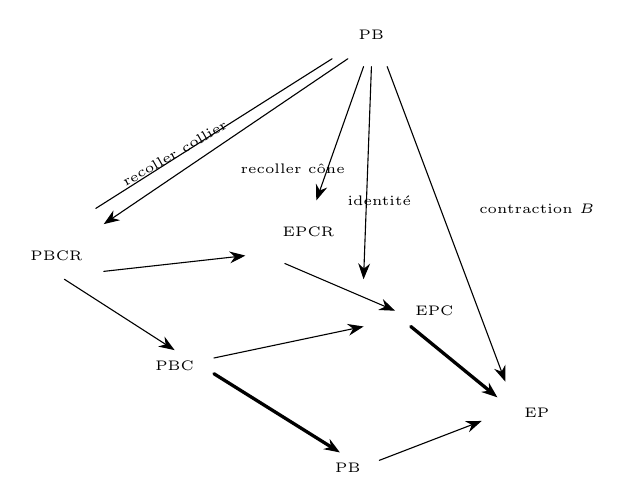
\begin{tikzpicture}[x=1mm,y=1mm,line cap=round,line join=round,font=\scriptsize]
\node[inner sep=1pt] at (65,-9) {\tiny $\mathrm{PB}$};
\node[inner sep=1pt] at (25,-37) {\tiny $\mathrm{PBCR}$};
\node[inner sep=1pt] at (57,-34) {\tiny $\mathrm{EPCR}$};
\node[inner sep=1pt] at (40,-51) {\tiny $\mathrm{PBC}$};
\node[inner sep=1pt] at (73,-44) {\tiny $\mathrm{EPC}$};
\node[inner sep=1pt] at (86,-57) {\tiny $\mathrm{EP}$};
\node[inner sep=1pt] at (62,-64) {\tiny $\mathrm{PB}$};
\draw[-{Stealth[length=2mm]}] (62,-12) -- (31,-33);
\draw (60,-12) -- (30,-31);
\draw[-{Stealth[length=2mm]}] (64,-13) -- (58,-30);
\draw[-{Stealth[length=2mm]}] (65,-13) -- (64,-40);
\draw[-{Stealth[length=2mm]}] (67,-13) -- (82,-53);
\draw[-{Stealth[length=2mm]}] (31,-39) -- (49,-37);
\draw[-{Stealth[length=2mm]}] (26,-40) -- (40,-49);
\draw[-{Stealth[length=2mm]}] (45,-50) -- (64,-46);
\draw[-{Stealth[length=2mm]}] (54,-38) -- (68,-44);
\draw[-{Stealth[length=2mm]},very thick] (70,-46) -- (81,-55);
\draw[-{Stealth[length=2mm]},very thick] (45,-52) -- (61,-62);
\draw[-{Stealth[length=2mm]}] (66,-63) -- (79,-58);
\node[inner sep=1pt,rotate=30] at (40,-24) {\tiny recoller collier};
\node[inner sep=1pt] at (55,-26) {\tiny recoller cône};
\node[inner sep=1pt] at (66,-30) {\tiny identité};
\node[inner sep=1pt] at (86,-31) {\tiny contraction $B$};
\end{tikzpicture}
\end{document}
